\documentclass{article}
\usepackage[utf8]{inputenc}
\usepackage{hyperref}

\usepackage[htt]{hyphenat}
\usepackage{epigraph}
\usepackage{fullpage}
\usepackage{graphicx}
\usepackage{dirtytalk}
\usepackage{float}
\parskip=5pt plus 1pt


\title{\textbf{Pogo Report}}
\author{Iván López Broceño}
\date{December 2021}

\begin{document}

\maketitle

\tableofcontents

\newpage
Remy's repo: \href{https://gitlab.u-angers.fr/remyguyonneau/pogo}{https://gitlab.u-angers.fr/remyguyonneau/pogo}

My repo with this documentation and some programs: \href{https://github.com/ivrolan/my_pogo}{https://github.com/ivrolan/my\textunderscore pogo}

\section{Setting the robot}

\subsection{Configuring the Raspberry Pi}
We will use \href{https://ubuntu.com/download/server}{Ubuntu Server 20.04} as the OS running in our Raspberry Pi. 

Download an image of the OS and flash it in a bootable SD with the tool of your preference. I've used \href{https://www.balena.io/etcher/}{Balena Etcher} but you can use other one, as the Raspberry Pi Imager.

Once the SD is flashed with our system, we can insert it in the Rpi and configure the system from an external monitor and keyboard. I had to insert this line to the \texttt{config.txt} to make it work with the monitor in the room 214.

\begin{verbatim}
hdmi_force_hotplug=1     
\end{verbatim}

\subsubsection{Credentials}
\label{Credentials} 
\begin{verbatim}
    user: ubuntu
    passwd: tubutubu
\end{verbatim}

\subsection{Wifi communication}

We have to set up also the wifi to let us connect to the robot even when it is moving (not attached to the router via Ethernet cable). We'll follow the documentation of Remy Guyonneau: \href{https://gitlab.u-angers.fr/remyguyonneau/pogo/-/blob/master/documentation/main.pdf}{https://gitlab.u-angers.fr/remyguyonneau/pogo/-/blob/master/documentation/main.pdf} - "Activation wifi - par point de access"

This should be already done and working.

After that, check the communication via ssh typing in your PC \textbf{connected to the same wifi that the robot}

I recommend setting a variable environment in your \verb|./bashrc| on your PC.
\begin{verbatim}
    export POGO_IP=192.168.1.13
\end{verbatim}

Test the ssh connection:

\begin{verbatim}
    ssh ubuntu@$POGO_IP
\end{verbatim}

And type the password\ref{Credentials}

\subsection{Installing and setting ROS environment}

\subsubsection{Installing ROS}
As we are on Ubuntu 20.04 we are going to use ROS noetic, precisely the \verb|ros-base| pkg.

\href{http://wiki.ros.org/noetic/Installation/Ubuntu}{Installation tutorial ROS Noetic on Ubuntu}

Remember to create a catkin workspace creating a directory with a \verb|src/| inside and compile it.

The SD already configured has the \verb|pogo_ws|

\subsubsection{Enabling the communication between the robot and your computer with ROS}

We have to set more environment variables. To communicate both machines, they have to be connected to the same \verb|roscore| and we have to "say" to our machines where is this \verb|roscore| setting the environment variables \verb|$ROS_MASTER_URI| and its own IP with \verb|$ROS_IP|.

I've configured it as it follows:

In the Raspberry Pi - robot:

\begin{verbatim}
    export ROS_MASTER_URI=http://192.168.1.13:11311/
    export ROS_IP=192.168.1.13
\end{verbatim}

In my own PC:

\begin{verbatim}
    export ROS_MASTER_URI=http://192.168.1.13:11311/
    export ROS_IP=$(ifconfig wlp2s0 | grep "inet " | awk '{print $2}') 
    # this allows us to get our own wifi IP from the wifi connection 
    # when we open a session in ssh
    export POGO_IP=192.168.1.13
\end{verbatim}

We can test this communication easily with:

In the robot:

\begin{verbatim}
    $ roscore
\end{verbatim}

In your PC:
\begin{verbatim}
    $ rostopic list
    /rosout
    /rosout_agg
\end{verbatim}

If an error pops out instead of getting the output of the topics, check that the \verb|roscore| is running with the correct IP in the robot.

\section{Support for the RPLIDAR sensor}

It was designed in Solidworks. Files can be found in 
\href{https://github.com/ivrolan/pogo-rplidar-case-files.git}{https://github.com/ivrolan/pogo-rplidar-case-files.git}

\begin{figure}[H]
    \centering
    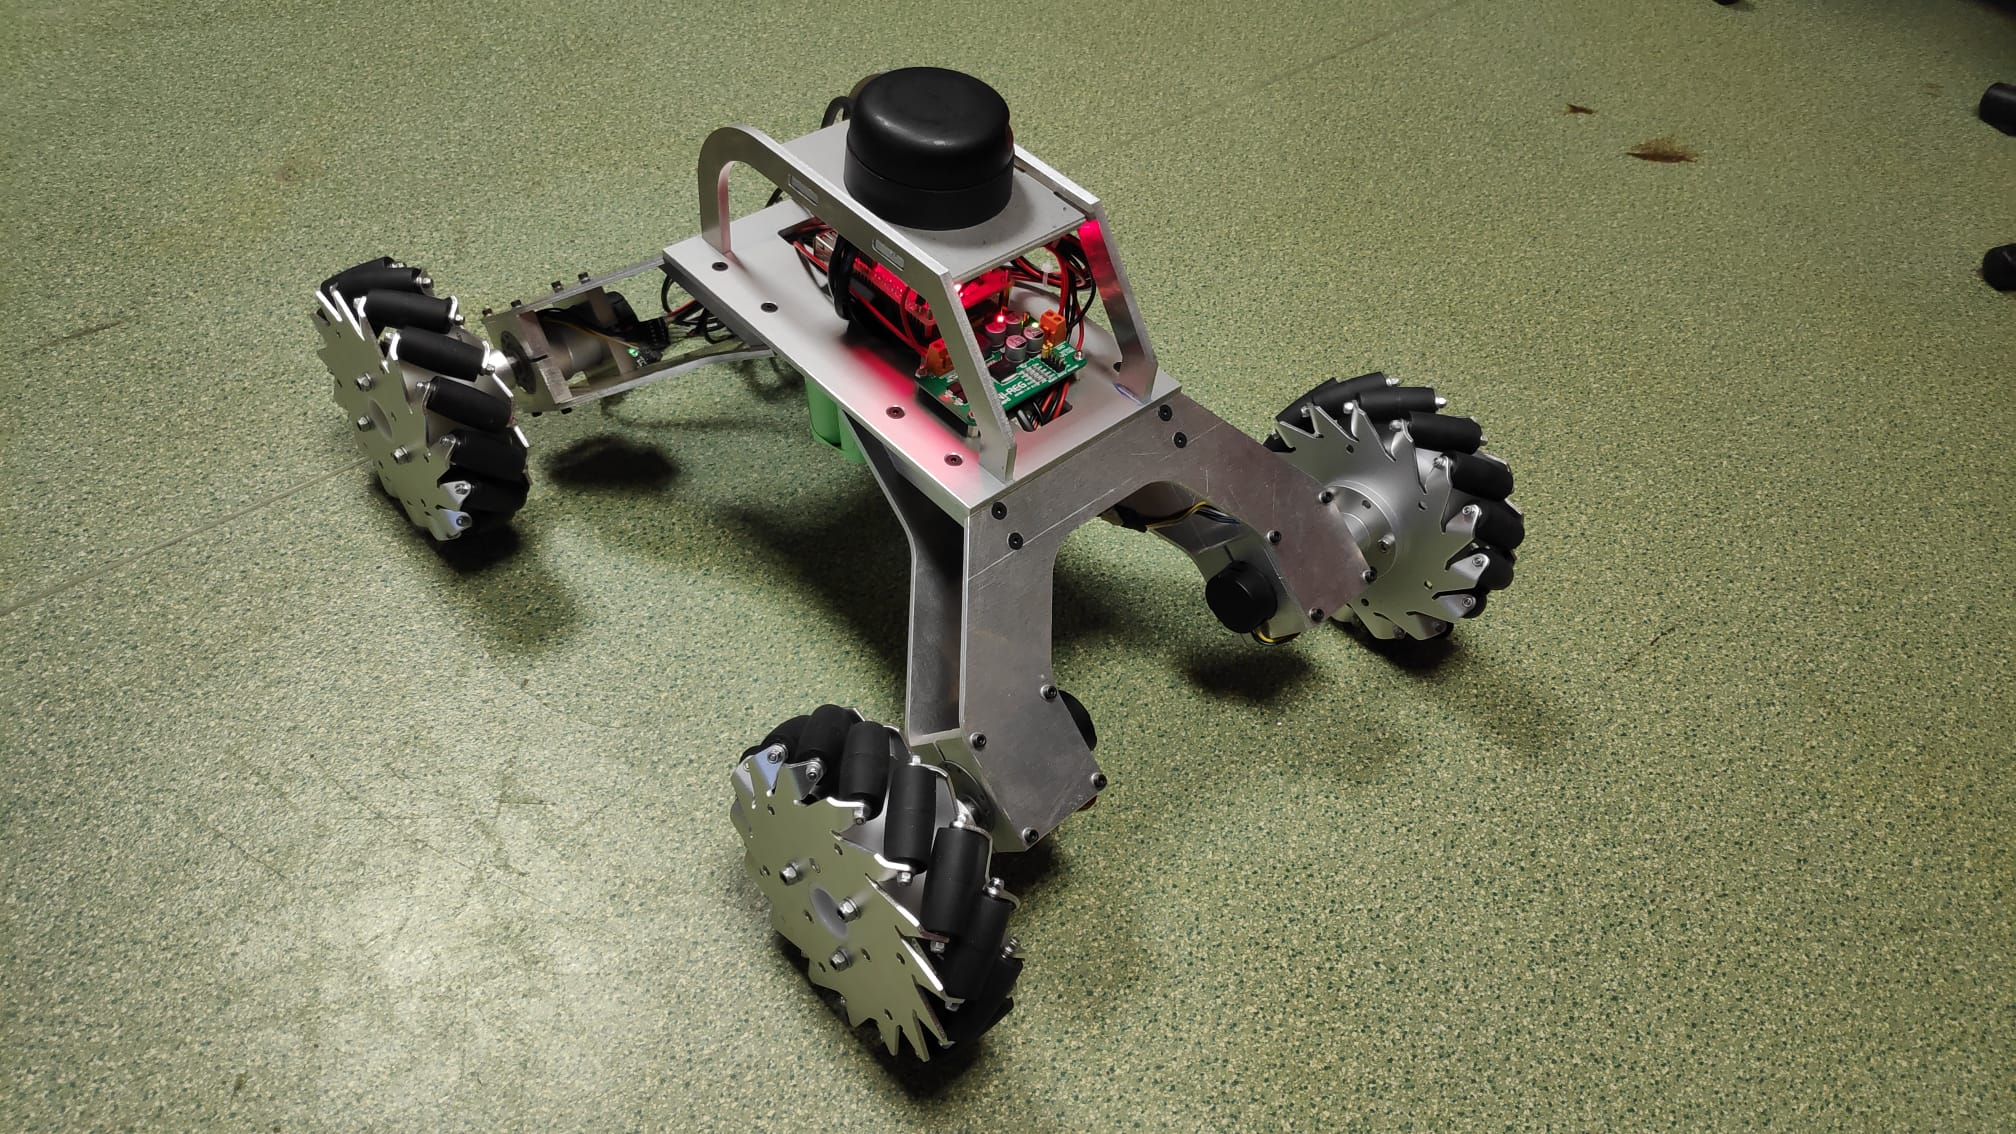
\includegraphics[width=\linewidth]{pogo_robot_full.jpeg}
    \caption{Full robot design.}
    \label{fig:fullroobot}
\end{figure}

\section{ROS code}
\subsection{Movement}
Nodes used to move the robot from the main repo of \href{https://gitlab.u-angers.fr/remyguyonneau/pogo}{Remy} and \href{https://github.com/ivrolan/my_pogo}{my repo} (files marked with a *):

\begin{itemize}
    
    \item To enable the motors and listen for jacobian velocities.
    \begin{itemize}
        \item \verb|pca9685_node|
        \item \verb|pid_node.py|
    \end{itemize}
    
    They can be launched with \verb|roslaunch pogo robot.launch|
    
    \item To transform the \verb|/secured_cmd_vel| topic of geometry\textunderscore msgs/Twist msgs to jacobian commands
    \begin{itemize}
        \item \verb|jacobian_node.py*|
    \end{itemize}
    
    \item To control the velocities with the keyboard:
    \begin{itemize}
        \item \verb|my_control.py*|
    \end{itemize}
    To increase/decrease the linear velocities use the key arrows. You can adjust the step of change in each tap changing the parameter inside the code. To increase/decrease the angular speed, press K or L. To stop the robot (put all velocities at 0) press the spacebar
    
\end{itemize}

In the robot:
\begin{verbatim}
    $ roslaunch pogo robot.launch
\end{verbatim}

In your PC:
\begin{verbatim}
    $ rosrun pogo jacobian_node.py
    $ rosrun pogo my_control.py
\end{verbatim}

\subsection{Sensing with the RPLIDAR}

The LIDAR sensor mounted in top of the robot is a RPLIDAR A2. The code to make it work can be found at \href{https://github.com/Slamtec/rplidar_ros}{Slamtec github rplidar\textunderscore ros}

Clone the repo in the \verb|src/| directory of your catkin workspace:
\begin{verbatim}
    $ git clone https://github.com/Slamtec/rplidar_ros
\end{verbatim}

\textbf{WARNING !!!}

Testing this package in the last version gave problems with the sensing. The system could receive data, but the max\textunderscore range was 0, and no points of the laser were displayed. 

This was due to the SDK update to the version 2.0. I have posted an \href{https://github.com/Slamtec/rplidar_ros/issues/67#issue-1064430009}{issue} on the repo, so in the future check that thread to see if the bug was solved. Until then, go back to the version 1.9 with a git checkout to a previous state.

\begin{verbatim}
    $ git checkout 36684a01dcee58ada142b9199c04158b1439a84e
\end{verbatim}

\verb|36684a01dcee58ada142b9199c04158b1439a84e| is the hash of the commit to upgrade to the v1.9 of the SDK. You can check that with the output of

\begin{verbatim}
    $ git log
    commit 36684a01dcee58ada142b9199c04158b1439a84e (HEAD)
    Author: kint <huasheng_zyh@163.com>
    Date:   Fri Aug 24 01:04:21 2018 -0700

    upgrade sdk 1.9.0
    [new feature] support baudrate 57600 and 1382400, support HQ scan response
    [bugfix] TCP channel doesn't work
    [improvement] Print warning messages when deprecated APIs are called; imporve angular accuracy for ultra capsuled scan points
\end{verbatim}

Once you have the package compiled in the right version you can test it on the robot (as it will take data from the USB it has to be executed on the robot):

\begin{verbatim}
    $ roslaunch rplidar_ros rplidar.launch
\end{verbatim}

And then in your pc:
\begin{verbatim}
    $ rviz
\end{verbatim}
And add the LaserPoint topic visualizer and set properly the frame to see the points published in the topic \verb|/scan|. Something like this

\begin{figure}[H]
    \centering
    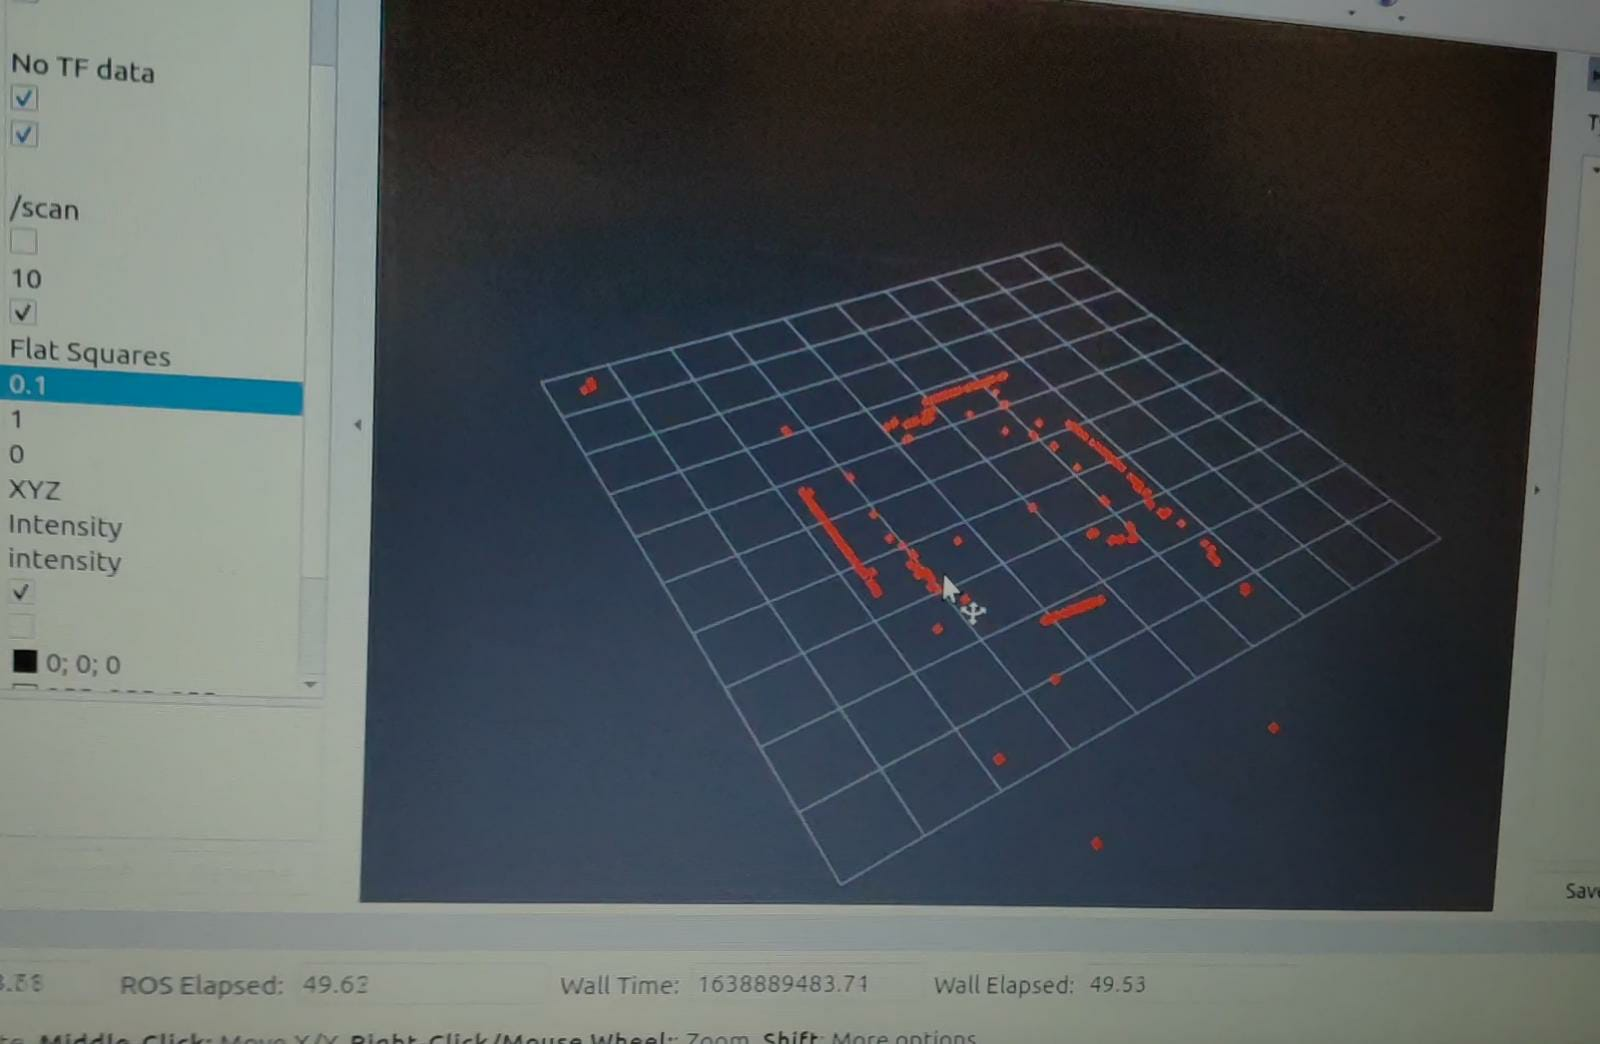
\includegraphics[scale=0.2]{laser.jpeg}
    \caption{Example of Lidar visualization}
    \label{fig:lidar_viz}
\end{figure}

\subsection{SLAM with hector\textunderscore slam package}

 Now that we have the lidar sensing working we can use it to create a map of the surroundings of the robot at the same time that we locate the robot in that map. Additionally to the lidar data, we also need the relation of positions between the proyection of the center of the robot in the floor and the lidar sensor.
 
 \subsubsection{Setting up the TF of the robot}
 
 The transforms (TF) state the relation between coordinate frames. All of those TF have to link the frames creating a tree (each frame has only one parentframe). 
 
 In this case of use,  the tree of transforms would be like:
 
 $ map \rightarrow base\textunderscore link \rightarrow laser $
 
 To do that, a \verb|tf_broadcaster| is created, that links \verb|base_link| with the \verb|laser| frame. This program can be found at  \href{https://github.com/ivrolan/pogo_setup_tf.git}{https://github.com/ivrolan/pogo\textunderscore setup\textunderscore tf.git}
 
 \begin{figure}[H]
    \centering
    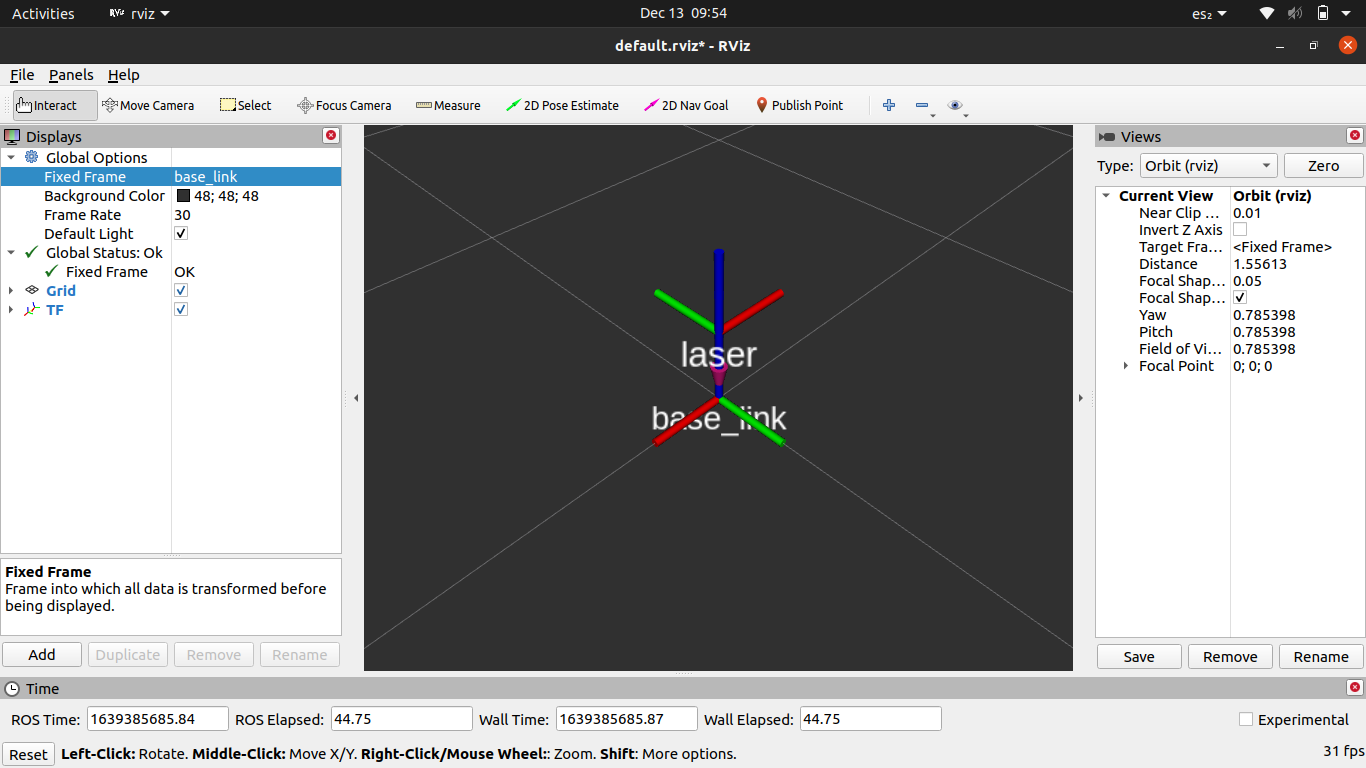
\includegraphics[width=\linewidth]{tf.png}
    \caption{How the tf should be linked thanks to tf\textunderscore broadcaster}
    \label{fig:tf}
\end{figure}
 
 \subsubsection{The hector\textunderscore slam package}
 
 The repo can be found at \href{https://github.com/tu-darmstadt-ros-pkg/hector_slam}{https://github.com/tu-darmstadt-ros-pkg/hector\textunderscore slam}.
 
 Changes:
 
 - In \verb|hector_slam_launch/launch/tutorial.launch| change the line 
 \begin{verbatim}
     <param name="/use_sim_time" value="true"/>
 \end{verbatim}
 by this one
 \begin{verbatim}
     <param name="/use_sim_time" value="false"/>
 \end{verbatim}
 
 
- Also in \verb|hector_mapping/launch/mapping_default.launch| we have to change:
\begin{verbatim}
    <arg name="tf_map_scanmatch_transform_frame_name" default="scanmatcher_frame"/>
    <arg name="base_frame" default="base_footprint"/>
    <arg name="odom_frame" default="nav"/>
\end{verbatim}

By:
\begin{verbatim}
    <arg name="tf_map_scanmatch_transform_frame_name" default="laser"/>
    <arg name="base_frame" default="base_link"/>
    <!-- If we don't want to use odom we have to change it name to the one in "base_frame"-->
    <arg name="odom_frame" default="base_link"/>
\end{verbatim}
 
Given all of that well configured we can test it like:

\begin{itemize}
    \item Launching the control of the movement with:
    \begin{itemize}
        \item ROBOT: \verb|roslaunch robot robot.launch|
        \item PC: \verb|rosrun pogo jacobian_node.py|
        \item PC: \verb|rosrun pogo my_control.py|
    \end{itemize}
    \item Launching the rplidar sensor
    \begin{itemize}
        \item ROBOT: \verb|roslaunch rplidar_ros rplidar.launch|
    \end{itemize}
    
    \item Running the hector slam
    \begin{itemize}
        \item PC: \verb|roslaunch hector_slam_launch tutorial.launch|
    \end{itemize}
\end{itemize}

And we can move the robot frame around a map created on the fly in rviz. For more information about hector slam see \href{https://wiki.ros.org/hector_slam}{https://wiki.ros.org/hector\textunderscore slam}.

\subsection{Navigation}

\subsubsection{With move\textunderscore base}
Now the goal is to use this map and localization provided by \verb|hector_slam| to navigate. We could use \href{http://wiki.ros.org/move_base}{move\textunderscore base} but I didn't succed to make it work with the map provided in real time by \verb|hector_slam|, \verb|move_base| was always using its own plugins to generate the maps, although the path created by its planner if a goal was selected in rviz and the commands to follow it seemed correct. 

\subsubsection{With hector\textunderscore navigation}
We tried also the \href{https://github.com/tu-darmstadt-ros-pkg/hector_navigation/tree/noetic-devel}{hector\textunderscore navigation pkg} 

Change the \verb|hector_navigation/hector_exploration_node/config/costmap.yaml| file to:

\begin{verbatim}
    global_costmap:

  map_type: costmap
  track_unknown_space: true
  unknown_cost_value: 255
  obstacle_range: 2.5
  raytrace_range: 3.0
  footprint: [[0.2, 0.26],
              [0.2, -0.26],
              [-0.2, -0.26],
              [-0.2, 0.26]]
  inflation_radius: 0.2
  #transform_tolerance: 0.5
  inscribed_radius: 0.3
  circumscribed_radius: 0.32

  global_frame: map
  robot_base_frame: base_link
  update_frequency: 0.5
  publish_frequency: 0.1
  static_map: true
  rolling_window: false

  #Investigate what this actually does
  cost_scaling_factor: 10.0

\end{verbatim}

Now you can run with the hector slam running:
\begin{verbatim}
    $ roslaunch hector_exploration_node exploration_planner.launch 
\end{verbatim}

To get goal poses and paths to follow to explore the area. To follow this path we can use the \verb|simple_exploration_controller| included in the \verb|hector_navigation| pkg.

With all the previously mentioned running (except the \verb|my_control.py| node):

\begin{verbatim}
    $ rosrun hector_exploration_controller simple_exploration_controller
\end{verbatim}

In my case, I didn't success using this node: the robot was kept turning in circles, without following the path given by the \verb|hector_exploration_planner|.

\begin{figure}[H]
    \centering
    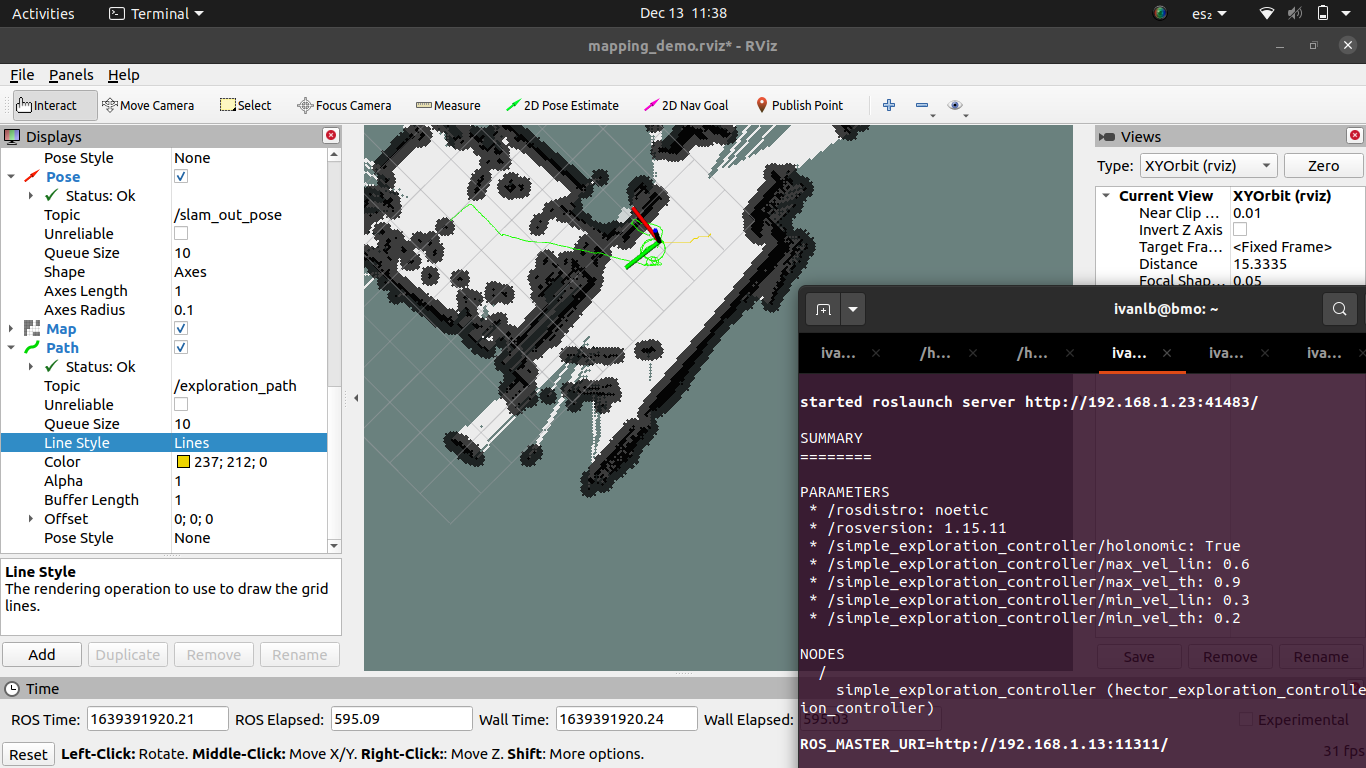
\includegraphics[width=\linewidth]{simple_controller.png}
    \caption{The robot doesn't follow the yellow line (the path given)}
    \label{fig:simple_exploration_controller}
\end{figure}


\section{Further details - Contact information}

This report was done by Iván López Broceño, student of Software Robotics Engineering at Universidad Rey Juan Carlos, Spain, during his Erasmus mobility at the Polytech Angers, France.  

Do not hesitate to contact me if more information, details or help are needed. I am willing to help as much as I can.
\begin{itemize}
    \item \textbf{Universidad Rey Juan Carlos email:} i.lopezb.2019@alumnos.urjc.es
    \item \textbf{University of Angers email:} ivan.lopezbroceno@etud.univ-angers.fr
    \item \textbf{Github:} \href{https://github.com/ivrolan}{https://github.com/ivrolan}
\end{itemize}


\end{document}
